\documentclass[a5paper,headsepline,titlepage,11pt,normalheadings,DIVcalc]{scrbook}
\usepackage[a5paper,backref]{hyperref}
\usepackage[papersize={148.5mm,215mm},twoside,bindingoffset=0.5cm,hmargin={2cm,2cm},
				vmargin={2cm,2cm},footskip=1.1cm,driver=dvipdfm]{geometry}
%\usepackage{palatino}
\usepackage{graphicx}
\usepackage{wrapfig}
\usepackage[bahasa]{babel}
\usepackage{fancyhdr}
\usepackage{pst-text}
\usepackage{pst-grad}
\usepackage{marvosym}

%\setlength{\voffset}{0.5in}
%\setlength{\oddsidemargin}{28pt}
%\setlength{\evensidemargin}{0pt}
\renewcommand{\footrulewidth}{0.5pt}
\lhead[\fancyplain{}{\thepage}]%
      {\fancyplain{}{\rightmark}}
\rhead[\fancyplain{}{\leftmark}]%
      {\fancyplain{}{\thepage}}
\pagestyle{fancy}
\lfoot[\emph{Misa peringatan 2 tahun \namaalm}]{}
\rfoot[]{\emph{Misa peringatan 2 tahun \namaalm}}
\cfoot{}

\makeatletter
\newcommand{\judul}[1]{%
  {\parindent \z@ \centering 
    \interlinepenalty\@M \Large \bfseries #1\par\nobreak \vskip 20\p@ }}
\newcommand{\subjudul}[1]{%
  {\parindent \z@ 
    \interlinepenalty\@M \bfseries #1\par\nobreak \vskip 10\p@ }}
\newcommand{\lagu}[1]{%
  {\parindent \z@ 
    \interlinepenalty\@M \slshape \mdseries \Large \textit{#1}\par\nobreak \vskip 10\p@ }}
\newcommand{\keterangan}[1]{%
  {\parindent \z@  \slshape 
    \interlinepenalty\@M \textsl{#1}\par\nobreak  \vskip 5\p@}}

\renewenvironment{description}
               {\list{}{\labelwidth\z@ \itemindent-\leftmargin
                        \let\makelabel\descriptionlabel}}
               {\endlist}
\renewcommand*\descriptionlabel[1]{\hspace\labelsep 
                                \normalfont\bfseries #1 }


\makeatother

\newcommand{\BU}[1]{\begin{itemize} \item[U:] #1 \end{itemize}}
\newcommand{\BI}[1]{\begin{itemize} \item[I:] #1 \end{itemize}}
\newcommand{\BIU}[1]{\begin{itemize} \item[I+U:] #1 \end{itemize}}
\newcommand{\BP}[1]{\begin{itemize} \item[P:] #1 \end{itemize}}
\newcommand{\inputlagu}[1]{\begin{textit} \input{#1} \end{textit}}
\newcommand{\namaalm}{Ibu Maria Goretti Ari Triwuryanti~}
\newcommand{\namaromo}{H Asodo OMI~}

\title{Misa Peringatan 2 tahun}
\author{\namaalm\\
(13 Februari 2010)}
\date{oleh \\ Rm \namaromo\\3 Maret 2012}
\hyphenation{sa-u-da-ra-ku}
\hyphenation{ke-ri-ngat}
\hyphenation{je-ri-tan}
\hyphenation{hu-bung-an}
\hyphenation{me-nya-dari}
\hyphenation{Eng-kau}
\hyphenation{ke-sa-lah-an}
\hyphenation{ba-gai-ma-na}
\hyphenation{Tu-han}
\hyphenation{di-per-ca-ya-kan}
\hyphenation{men-ja-uh-kan}
\hyphenation{bu-kan-lah}
\hyphenation{per-sa-tu-kan-lah}
\hyphenation{ma-khluk}
\hyphenation{Sem-buh-kan-lah}
\hyphenation{ja-lan}
\hyphenation{mem-bu-tuh-kan}
\hyphenation{be-ri-kan-lah}
\hyphenation{me-ra-sa-kan}
\hyphenation{te-man-ilah}
\hyphenation{mem-bi-ngung-kan}
\hyphenation{di-ka-gum-i}
\hyphenation{ta-ngis-an-Mu}
\hyphenation{mi-lik-ilah}


\begin{document}
%\maketitle
\thispagestyle{empty}
\newsavebox\IBox
\sbox\IBox{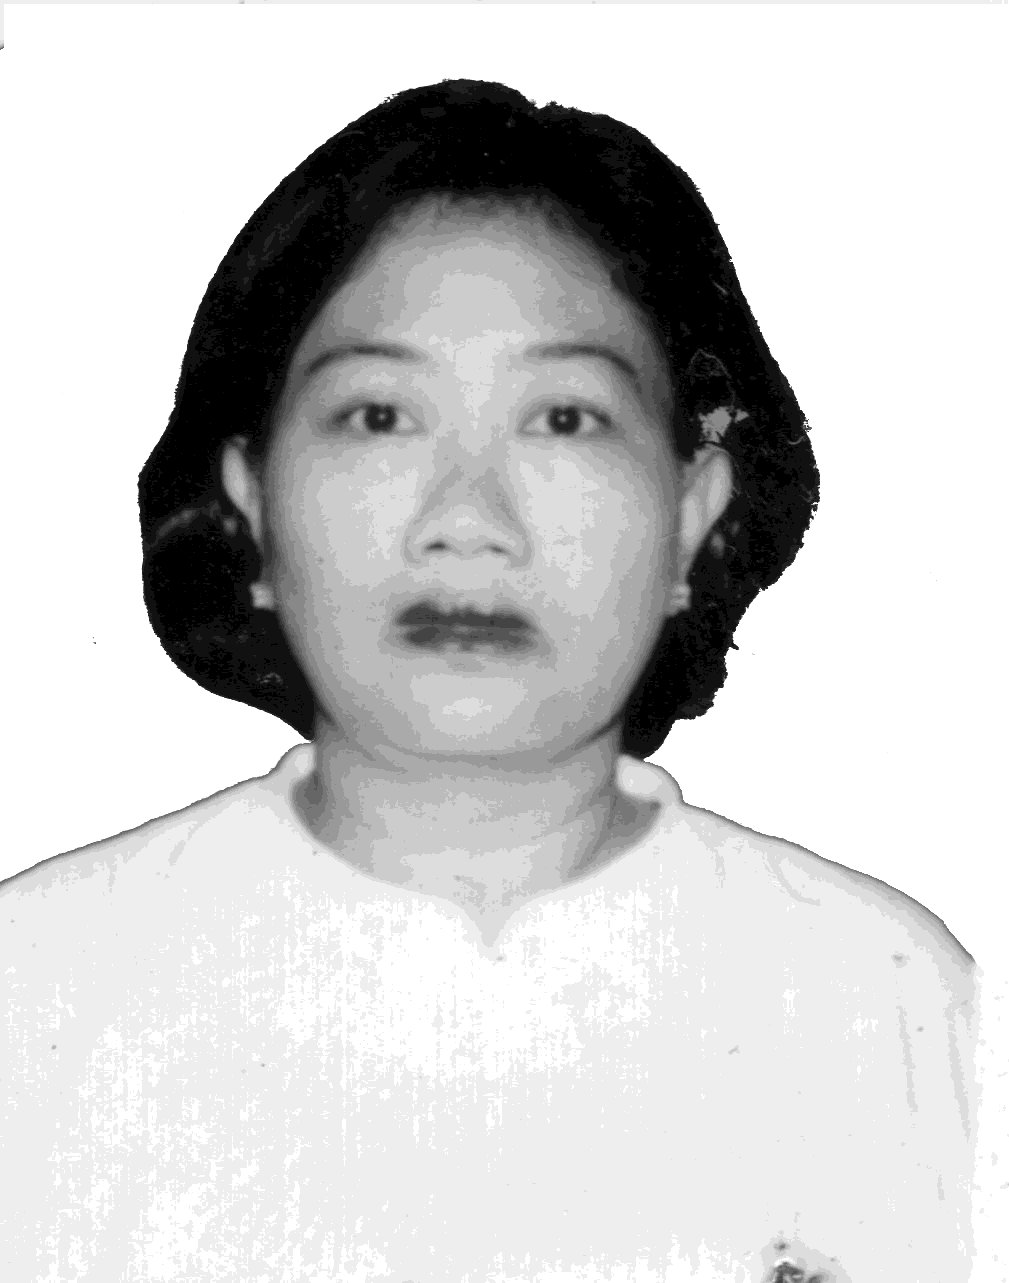
\includegraphics[scale=2]{gambar/sri3.jpg}}
% set up the picture environment
\psset{unit=1in}
\begin{pspicture}(4in,5in)
% set up the fonts we use
\DeclareFixedFont{\PT}{T1}{ppl}{b}{it}{0.5in}
\DeclareFixedFont{\PTsmall}{T1}{ppl}{b}{it}{0.4in}
\DeclareFixedFont{\PTsmaller}{T1}{ppl}{b}{it}{0.3in}
\DeclareFixedFont{\PTsmallest}{T1}{ppl}{b}{it}{0.2in}
\DeclareFixedFont{\PTtext}{T1}{ppl}{b}{it}{11pt}
\DeclareFixedFont{\Logo}{T1}{pbk}{m}{n}{0.3in}
% place the front cover picture
\rput[cb](2,1.25){\usebox\IBox}
% put the text on the front cover
\rput[cb](2,4.5){\PTsmall {Ekaristi}}
\rput[cb](2,4.1){\PTsmall {Peringatan 2 tahun}}
\rput[cb](2,3.0){\PTsmaller {\namaalm}}
\rput[cb](2,2.6){\PTsmallest(1 Maret 2010)}
\rput[cb](2,-0.4){\PTsmallest {oleh}} 
\rput[cb](2,-0.8){\PTsmallest {Rm \namaromo}}
\rput[cb](2,-1.2){\PTsmallest {3 Maret 2012}}

%\rput[cb](3,-1){\PTsmallest {\namagereja}} 

\end{pspicture}

\newpage
\thispagestyle{empty}
{~}
\newpage

\section*{RITUS PEMBUKA} 

 

\lagu{Lagu Pembuka}  
%\begin{center}
Ya Tuhan Pandang HambaMu
\end{center}

\begin{verse}
Ya Tuhan pandang hambaMu \\
yang sujud menyembah.\\
Penuh syukur kepadaMu \\
dan hati berserah.\\
\end{verse}

\begin{verse}
Sembah dan bakti umatMu\\ 
pujian kemuliaanMu\\
seutuhnya terimalah \\
dan ampunMu limpahkanlah\\
Berpalinglah kepada hambaMu
\end{verse}

 

\subjudul{Tanda Salib} 

\BI{Demi nama  Bapa dan Putera dan Roh Kudus}

\BU{Amin}

 

\subjudul{Salam}

\BI{Semoga kasih karunia, rahmat dan damai sejahtera dari 
Allah Bapa dan dari PuteraNya Yesus Kristus beserta 
saudara.} 

\BU{Sekarang dan selama-lamanya.}

 

\subjudul{Pengantar}

\BI{Terpujilah Allah Bapa di surga: Ia yang memiliki, Ia yang 
memberi dan memelihara, Ia pula yang mengambilnya 
kembali. Terpujilah Allah Bapa di surga.

\namaalm adalah milik Bapa di surga. Karena kasihNya 
kepada kita semua, kita telah menikmati kehadirannya.
KepadaNya pulalah dia telah 
kembali.

Kini kita bersama-
sama berdoa menghadap Allah Bapa di surga untuk 
bersyukur atas kehadirannya, atas teladan kehidupannya 
dan memohon berkat Allah untuk arwahnya 
agar supaya Allah Bapa berkenan mengampuni dosa-dosanya 
dan menerimanya dalam rumah abadi dalam 
damai dan kemuliaan Allah Bapa di surga. 

Kita juga memohon kepada Allah Bapa untuk berkatNya 
agar kita dapat meneruskan kebiasaan baik dari \namaalm , 
terutama dalam kehidupan spiritualitas dan 
sosialitas kita.}

 

\subjudul{Tobat}

\BI{Tuhan Yesus, Engkau mengalami kematian sebagai manusia tetapi dibangkitkan oleh kekuasaan Bapa dalam Roh Kudus.

Tuhan kasihanilah kami}

\BU{Tuhan kasihanilah kami}

\BI{Engkaulah kebangkitan dan kehidupan, barang siapa percaya kepadaMu akan memperoleh kehidupan yang kekal.

Kristus kasihanilah kami}

\BU{Kristus kasihanilah kami}

\BI{Engkau akan datang kembali dengan mulia untuk mempersatukan kami semua dalam kerajaan surga.

Tuhan kasihanilah kami}

\BU{Tuhan kasihanilah kami}

\BI{Semoga Allah Bapa yang Maha Kuasa, mengasihani kita, 
mengampuni dosa kita dan mengantar kita ke dalam 
kehidupan kekal.}

\BU{Amin}

 

\subjudul{Doa Pembuka}

\BI{Marilah kita berdoa 

Allah Bapa yang mahamurah, Engkau telah menebus dosa
kami dengan wafat dan kebangkitan Putra-Mu terkasih.
Kasihanilah kiranya hambaMu, saudara kami \namaalm yang sudah
Engkau panggil 2 tahun yang lalu. Saudara kami \namaalm percaya
bahwa setelah kematian ada kebangkitan dan kehidupan abadi
di surga. Semoga saudara kami ini juga Engkau perkenankan
untuk menikmati kebahagiaan kekal abadi di surga. Demi
Yesus Kristus, Putra-Mu, Tuhan dan pengantara kami, yang
bersatu dengan Dikau dan Roh Kudus hidup dan berkuasa kini
dan sepanjang masa.
}

\BU{Amin}

 

\section*{LITURGI SABDA} 

\keterangan{Pembacaan dari Surat Rasul Paulus kepada umat di Kolose
(1:12-20)}

\BU{Saudara-saudari, marilah kita mengucap syukur dengan suka cita kepada
Bapa, yang melayakkan kamu untuk mendapat bagian dalam
apa yang ditentukan untuk o-rang-orang kudus di dalam kerajaan
terang. Ia telah melepaskan kita dari kuasa kegelapan dan
memindahkan kita ke dalam Kerajaan Anak-Nya yang kekasih;
di dalam Dia kita memiliki penebusan kita, yaitu pengampunan
dosa. Ia adalah gambar Allah yang tidak kelihatan, yang
sulung, lebih utama dari segala yang diciptakan, karena di
dalam Dialah telah diciptakan segala sesuatu, yang ada di sorga
dan yang ada di bumi, yang kelihatan dan yang tidak kelihatan,
baik singgasana, maupun kerajaan, baik pemerintah, maupun
penguasa; segala sesuatu diciptakan oleh Dia dan untuk Dia. Ia
ada terlebih dahulu dari segala sesuatu dan segala sesuatu ada
di dalam Dia. Ialah kepada tubuh, yaitu jemaat. Ialah kepala
tubuh, yaitu jemaat. Ialah yang sulung, yang pertama bangkit
dari antara orang mati, sehingga Ia yang lebih utama dalam
segala sesuatu. Karena seluruh kepenuhan Allah berkenan diam
di dalam Dia, dan oleh Dialah Ia memperdamaikan segala
sesuatu dengan diri-Nya, baik yang ada di bumi, maupun yang
ada di sorga, sesudah Ia mengadakan pendamaian oleh darah
salib Kristus.

Demikianlah Sabda Tuhan}

\BU{Syukur kepada Allah}
\subjudul{Bacaan Injil}

\BI{Tuhan sertamu}

\BU{dan sertamu juga} 

\BI{Inilah Injil Yesus Kristus menurut Yohanes (5:24-29)}

\BU{Dimuliakanlah Tuhan}

\BI{Aku berkata kepadamu : Sesungguhnya barangsiapa
mendengar perkataan-Ku dan percaya kepada Dia yang
mengutus Aku, ia mempunyai hidup yang kekal dan tidak
turut dihukum, sebab ia sudah pindah dari dalam maut ke
dalam hidup. Aku berkata berkata kepadamu :
Sesungguhnya saatnya akan tiba dan sudah tiba, bahwa
orang-orang mati akan mendengar suara Anak Allah, dan
mereka yang mendengarnya, akan hidup. Sebab sama
seperti Bapa mempunyai hidup dalam diri-Nya sendiri,
demikian juga diberikan-Nya Anak mempunyai hidup
dalam diri-Nya sendiri. Dan Ia telah memberikan kuasa
kepada-Nya untuk menghakimi, karena Ia adalah Anak
Manusia. Janganlah kamu heran akan hal itu, sebab saatnya
akan tiba, bahwa semua orang yang di dalam kuburan akan
mendengar suara-Nya, dan mereka yang telah berbuat baik
akan keluar dan bangkit untuk hidup yang kekal, tetapi
mereka yang telah berbuat jahat akan bangkit untuk
dihukum.

Demikianlah Injil Tuhan}

\BU{Terpujilah Kristus.}

 

\subjudul{Homili}

\subjudul{Syahadat} 

\subjudul{Doa Umat}

\BI{Terpujilah Engkau ya Allah Bapa di surga karena besarlah kuasa 
dan kasihMu. Kami menghaturkan puji dan sembah atas segala 
kurnia yang telah Engkau limpahkan kepada kami: atas keluarga 
kami; atas rumah tempat tinggal kami; atas segala sesuatu yang 
telah kami terima dan nikmati mulai dari doa, teladan, seluruh 
kebutuhan hidup dan pendidikan yang Engkau berikan melalui 
orang-orang yang mengasihi kami.}

\BP{Bagi keselamatan saudara kita \namaalm
Semoga berkat kesetiaannya kepada Yesus sang Penebus
dan Penyelamat kita, saudara kita \namaalm dihantar dan
dianugerahi masuk ke dalam kerajaan-Nya untuk
menikmati kedamaian abadi.

Marilah kita mohon \ldots}

\BU{Kabulkanlah doa kami, ya Tuhan}

\BP{Bagi keselamatan jiwa Bapak Adi Anggono yang telah berpulang: Semoga ia diberi tempat yang layak di dalam Kerajaan Surga

Marilah kita mohon \ldots}

\BU{Kabulkanlah doa kami, ya Tuhan} 

\BP{Bagi kita yang hadir di sini:
Semoga Kristus Penyelamat kita menghancurkan
kekuasaan dosa supaya kita juga layak menerima hidup
abadi dalam Dia.

Marilah kita mohon \ldots}

\BU{Kabulkanlah doa kami, ya Tuhan}

\BP{Bagi semua yang sedang berdukacita:
Semoga Kristus penghibur orang yang berdukacita
menghapuskan air mata serta dukacita dari hati orang-
orang yang sedang berkabung karena kehilangan sanak
saudara mereka.

Marilah kita mohon \ldots}

\BU{Kabulkanlah doa kami, ya Tuhan}

\BP{Bagi semua orang yang percaya kepada Kristus :
Semoga semua orang yang percaya kepada Kristus kelak
pada akhir zaman berbahagia dan bersatu dalam surga
abadi dengan semua orang yang telah meninggal dalam
iman kepada-Nya.

Marilah kita mohon \ldots}

\BU{Kabulkanlah doa kami, ya Tuhan}

\BI{Allah yang kekal dan kuasa, semoga dalam kerahimanMu beristirahatlah arwah semua orang orang beriman, terutama saudara-saudari yang kami kenang saat ini. Kabulkanlah doa kami. Demi Kristus, Tuhan dan Juruselamat kami, kini dan sepanjang masa.}

\BU{Amin.}

\section*{LITURGI EKARISTI}

\lagu{Lagu Persembahan}

\BI{Kami memuji Engkau ya Bapa, Allah semesta alam, sebab 
dari kemurahanMu kami menerima roti dan anggur yang 
kami persembahkan ini. Inilah hasil dari bumi dan usaha 
manusia yang bagi kami akan menjadi santapan rohani.}

\BU{Terpujilah Allah selama-lamanya}

\BI{Berdoalah saudara-saudara supaya persembahan kita ini 
diterima oleh Allah Bapa yang mahakuasa.}

\BU{Semoga persembahan ini diterima demi kemuliaan Tuhan 
dan keselamatan kita serta seluruh umat Allah yang kudus.}

\BI{Ya Allah Bapa di surga, pengampunanMu menjadi sumber 
kedamaian dan kekuatan baru di dalam hati kami untuk 
mengikuti PuteraMu dengan setia. Maka kami mohon 
pandanglah dengan rela persembahan di atas altar ini dan 
teguhkanlah hati kami berkat korban Yesus Kristus, Tuhan 
dan Pengantara kami kini dan sepanjang masa.}

\BU{Amin} 

\subjudul{DOA SYUKUR AGUNG}

\subjudul{Bapa Kami}

\subjudul{Komuni}

\subjudul{Lagu Komuni}
 
\subjudul{Doa sesudah komuni}

\BI{Marilah berdoa: 

Tuhan Yesus Kristus, bantulah kami dan bimbinglah kami
dengan Roh Kudus-Mu, supaya kami selalu mendengar,
percaya dan menghidupi sabdaMu. Hantarkanlah kami
semua dalam ziarah hidup ini agar sampai ke rumah-Mu
dan kelak bersatu kembali dengan saudara-saudari kami
yang sudah mendahului kami. Sebab Engkaulah Tuhan
dan Perantara kami.
}

\BU{Amin.}

\section*{RITUS PENUTUP}

\BI{Tuhan sertamu}

\BU{dan sertamu juga}

\BI{Semoga saudara sekalian diberkati oleh Allah Bapa yang 
mahakuasa \Cross ~Bapa dan Putera dan Roh Kudus.}

\BU{Amin}

 

\subjudul{Pengutusan}

\BI{Saudara sekalian, Perayaan Ekaristi untuk memohon 
berkat Allah Bapa bagi arwah \namaalm serta seluruh leluhur dan anggota keluarga yang 
telah meninggal dunia telah selesai.}

\BU{Syukur kepada Allah}

\BI{Kita diutus untuk mewartakan bahwa Tuhan Yesus adalah 
jalan, kebangkitan dan hidup.}

\BU{Amin.}

 

\lagu{Lagu Penutup}


\newpage
\begin{flushright}
{\Large Ucapan terima kasih}
\noindent Dengan penuh syukur dalam kasih Tuhan, kami mengucapkan banyak
terima kasih kepada:
\large

\textbf{Romo \namaromo}\\
yang telah berkenan mempimpin perayaan ekaristi peringatan 2 tahun meninggalnya \namaalm
ini.

\textbf{Umat lingkungan Santo Petrus Maguwo dan tamu undangan}\\
yang telah mendukung perayaan ekaristi ini.

\textbf{Segenap keluarga dan orang-orang terkasih}\\
yang telah berkenan hadir memberikan cinta dan doa dalam perayaan
ekaristi ini.

Semoga Tuhan memberkati dan memelihara ikatan kasih\\ di antara kita semua.

Amin.

\bigskip 

Asri Anggarini\\
Asri Wuryantari\\
dan segenap keluarga
\end{flushright}

\end{document} 
